\documentclass{beamer}
\usetheme[hideothersubsections]{HRTheme}
\usepackage{beamerthemeHRTheme}
\usepackage{graphicx}
\usepackage[space]{grffile}
\usepackage{listings}
\lstset{language=SQL,
basicstyle=\ttfamily\footnotesize,
mathescape=true,
keywordstyle=\color{blue},
breaklines=true,
escapeinside={\%*}{*)}}
\usepackage[utf8]{inputenc}
\usepackage{color}
\newcommand{\red}[1]{
\textcolor{red}{#1}
}
\newcommand{\ts}{\textbackslash}

\title{Object-Relation Mapping}

\author{ }

\institute{Hogeschool Rotterdam \\ 
Rotterdam, Netherlands}

\date{}

\begin{document}
\maketitle

\SlideSection{Introduction}
\SlideSubSection{Lecture topics}
\begin{slide}{
\item Recap Java Database Connectivity  
\item Object-Relation Mapping.
\item Java Persistence API
\item Setting up JPA with EclipseLink.
}\end{slide}



\SlideSection{Object-Relation Mapping}
\SlideSubSection{JDBC}
\begin{slide}{
\item Provides a set of Java API for accessing the relational databases from Java program.
\item It allows querying/updating database data 
\item JDBC represents statements using one of the following classes:
\begin{enumerate}
	\pause
	 \item Statement – the statement is sent to the database server each and every time.
	 \pause
	 \item PreparedStatement – the statement is cached and then the execution path is pre-determined on the database server allowing it to be executed multiple times in an efficient manner.
	 \pause
	 \item CallableStatement – used for executing stored procedures on the database.
\end{enumerate}
}
\end{slide}



\SlideSubSection{Sample Code JDBC}
{
\begin{lstlisting}[language=java][showstringspaces=false]
..
try (Connection conn = DriverManager.getConnection(
	     "jdbc:somejdbcvendor:other data needed by some jdbc vendor",
	     "myLogin",
	     "myPassword" ) ) {
		
	Statement stmt = conn.createStatement()
	stmt.executeUpdate( "INSERT INTO Ships( name ) VALUE ( 'destroyer XYZ' ) " );
	}
 }  
..	
\end{lstlisting}	
}


\SlideSubSection{Disadvantages of JDBC}
\begin{slide}{
\item Less maintainable code for large projects
\item Queries are DBMS specific
}
\end{slide}

\SlideSubSection{ORM}
\begin{slide}{
\item It's a technique to map object state to the database columns
\pause
\item Hides details of SQL queries from OO logic.
\pause 
\item It provides a way for data conversion between incompatible type systems 
\pause 
\item Portability: DB independent
\pause 
\item Performance: Object and query caching mechanism  
\pause 
\item ORM are not only related to Java, other languages provide this technique
\begin{itemize}
\item C\#: Linq or Entity-Framework
\item Ruby: Active Record
\item Java Hibernate, EclipseLink
\end{itemize}
}
\end{slide}


\SlideSubSection{ORM and Data Persistence Strategies}
\begin{slide}{
\item There are some strategies designed for persistence of objects
\item ORM framework are based on those strategies (also called pattern) and framework specific implementations
\item Only two data persistence strategies will be discussed in this lecture
\pause 
\begin{itemize}
\item Active record
\item Data mapper 
\end{itemize}
}\end{slide}

\SlideSubSection{Active Record Strategy}
\begin{slide}{
\item In this strategy there is an object for every table or view that wraps a row
\pause
\item Objects structures are tightly coupled to the relational schema
\pause
\item This object encapsulates the database access, and adds domain logic on that data
\pause
\item So this object carries both data and behavior 

}\end{slide}


\SlideSubSection{Active Record Strategy}
\begin{slide}{
\item sample structure of active record 
\\
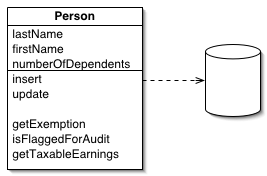
\includegraphics[scale=0.3]{img/activeRecordSketch.png}
}\end{slide}


\SlideSubSection{Active Record Strategy}
\begin{slide}{
\item What are the limitations of this pattern regarding objects structure? 
\pause
\item Think of domain object models that are distinguish from the one of the database schema
}\end{slide}


\SlideSubSection{Data Mapper Strategy}
\begin{slide}{
\item In strategy there is a layer of mappers that moves data between objects and a database 
\item This layer keeps both in-memory objects and database independent from each others 
\item The reasons for this are:
\pause
\begin{itemize}
\item Objects and relational databases have different mechanisms for structuring data
\pause
\item Many parts of an object, such as collections and inheritance, aren't present in relational databases
\item Object schema and database schema do not match in many cases
\end{itemize}
}\end{slide}


\SlideSubSection{Data Mapper}
\begin{slide}{
\item sample structure of data mapper 
\\
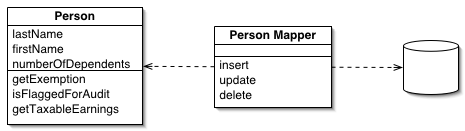
\includegraphics[scale=0.4]{img/databaseMapperSketch.png}
}\end{slide}



\SlideSubSection{Java Persistence API}
\begin{slide}{
\item Provides the standard specification for managing the relational data in applications
\item JPA is a layer between third party ORM implementations (EclipseLink or Hibernate) and the application 
\item It uses persistence annotations at three different levels: class, method, and field
\\
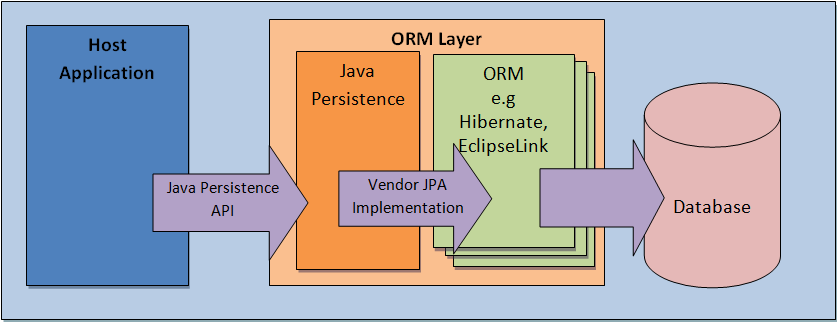
\includegraphics[scale=0.3]{img/JPA.png}
}
\end{slide} 


\begin{frame}[fragile]
Example of using annotation instead of mapping files 
\begin{lstlisting}[language=java]
import javax.persistence.*;

@Entity
@Table(name = "ships")
public class Ships {
   @Id @GeneratedValue
   @Column(name = "serial")
   private int serial;

   @Column(name = "name")
   private String name;

   @Column(name = "armour")
   private String armour; 

   public Employee() {}
   
   ...
   \end{lstlisting} 
\end{frame}


\begin{frame}[fragile]
Sample code for persisting a new ship in JPA with Hibernate 
\begin{lstlisting}[language=java]
....	 
Ships s = new Ships("Some ship name","metal");
....
EntityManagerFactory emf = Persistence.createEntityManagerFactory("InfDev5PU");
//create a session object in case of Hibernate
EntityManager em = emf.createEntityManager();
//starts a transaction 
em.getTransaction().begin();
//calls the save method of Hibernate
em.persist(em);
em.getTransaction().commit();
em.close();
....
\end{lstlisting} 
\end{frame} 
 

\SlideSubSection{Mapping Tables and Relationships in ORM}
\begin{slide}{
\item Mapping Simple Types like primitive java types: byte, int, short, etc.
\item Mapping tables to entity classes.
\item Mapping relationships: 
\begin{itemize}
\item In entity-classes the many-side of a relation can be mapped as Collections, Lists, Maps and Sets
\item It depends on the requirements within your application
\item Two entities cannot share a reference to the same collection instance  
\item There are special annotations (ex. @OneToMany) to support mappings
\end{itemize} 
}
\end{slide}  

\SlideSubSection{Lab}
\begin{slide}{
\item Check the tables mentioned in les 0
\item Create these tables in Postgres
\item Insert some new data into the database using JPA	
\item Print these data in your terminal using a named query 
}\end{slide}

\end{document}
